\input{preamble}
\usepackage{graphicx,wrapfig}
\usepackage{tkz-tab}
\usepackage{varwidth}
\graphicspath{ {./images/} }
\usetikzlibrary {datavisualization.formats.functions}

\begin{document}

\pagestyle{fancy}
\fancyhead[L]{Terminale STMG}
\fancyhead[C]{\textbf{TD n°4 : fiche méthode n°1}}
\fancyhead[R]{\today}

\exe{}{
Il faut connaître les règles de dérivation des polynômes et de la fonction inverse. \newline
\underline{Pour les polynômes :} on dérive chaque terme en $x$ (les \og monômes \fg), en retenant :
\begin{enumerate}
\item $ax^3$ se dérive en $3ax^2$ ;
\item $bx^2$ se dérive en $2bx$ ;
\item $cx$ se dérive en $c$ ;
\item $d$ se dérive en 0 (donc \og disparaît \fg).
\end{enumerate}  
En assemblant le tout, $x \mapsto ax^3 + bx^2 +cx + d$ se dérive en $x \mapsto 3ax^2 + 2bx + c$. \newline
\underline{Pour la fonction inverse :} la fonction $x \mapsto \frac{a}{x}$ se dérive en $x \mapsto -\frac{a}{x^2}$ 
(bien penser à \textbf{changer le signe}). \newline
\underline{Application :} 
\begin{enumerate}
\item la dérivée de $x \mapsto \frac7{x} + 3x$ est la fonction $x \mapsto -\frac7{x^2} + 3$.
\item la dérivée de $x \mapsto 4x^2 - 2x - \frac3{x}$ est la fonction $x \mapsto 8x -2 + \frac3{x^2}$.
\item la dérivée de $x \mapsto \frac3{2x} + x$ est la fonction $x \mapsto -\frac3{2x^2} + 1$.
\item  la dérivée de $x \mapsto 8x^3 - 7x^2 + 6x -2 - \frac{12}{x}$ est la fonction $x \mapsto 24x^2 -14x + 6 + \frac{12}{x^2}$.
\end{enumerate}
}{exe:1}{

}

\exe{}{
Pour étudier les variations de fonctions polynômes de degré 2, on procède ainsi :
\begin{enumerate}
\item On dérive la fonction polynôme.
\item On cherche les valeurs $x$ telles que la dérivée est nulle.
\item On cherche le signe de $f'(x)$ pour un $x$ donné.
\item On dresse le tableau de variation.
\end{enumerate}
\underline{Application :} 
\begin{enumerate}
\item On étudie les variations de la fonction $f:x \mapsto 2x^2 - 8x + 25$.
On a $f'(x) = 4x - 8$. On cherche $x$ tel que $f'(x)=0$.
\begin{align*}
f'(x) = 0 & \iff 4x - 8 = 0 \\
& \iff 4x = 8 \\
& \iff x = \dfrac84 \\
& \iff x = 2
\end{align*}
Pour connaître le signe de $f'(x)$ en fonction de $x$, on teste une valeur différente de celle trouvée précédemment.
Prenons par exemple $x=1, f'(1) = 4 - 8 = -4$ donc $f'(x) <0$ pour $x<2$.
On dresse maintenant le tableau de variation.
\begin{center}
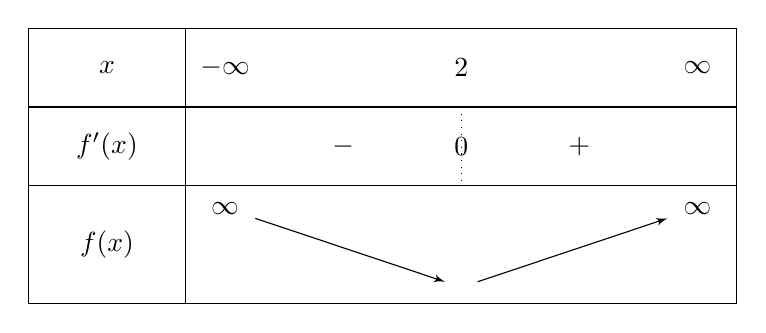
\begin{tikzpicture}
   \tkzTabInit{$x$ / 1 , $f'(x)$ / 1, $f(x)$ / 1.5}{$-\infty$, $2$, $\infty$}
   \tkzTabLine{, -, z, +, }
   \tkzTabVar{ +/ $\infty$, -/ , +/$\infty$ }
\end{tikzpicture}
\end{center}
On peut même calculer le minimum de $f$, qui est atteint en $2$ et qui vaut : 
\[ f(2) = 2 \cdot (2)^2 - 8 \cdot 2 + 25 = 17 . \]
\item $f:x \mapsto 4x^2 - 2x + \frac73, f'(x) = 8x -2 \et f'(x) = 0 \iff x = \frac14$. \newline
On remarque que $f'(1)=6 >0$.
\begin{center}
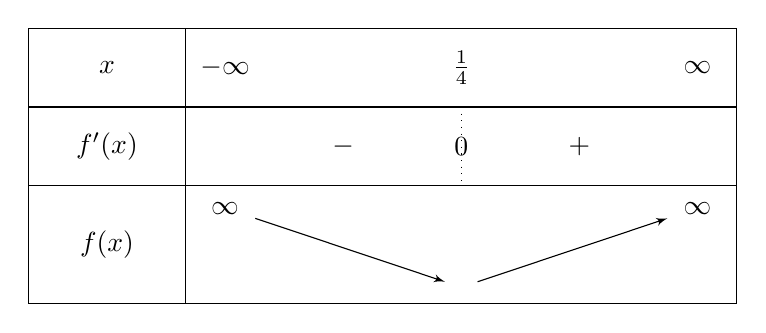
\begin{tikzpicture}
   \tkzTabInit{$x$ / 1 , $f'(x)$ / 1, $f(x)$ / 1.5}{$-\infty$, $\frac14$, $\infty$}
   \tkzTabLine{, -, z, +, }
   \tkzTabVar{ +/ $\infty$, -/ , +/$\infty$ }
\end{tikzpicture}
\end{center}
\item $f:x \mapsto \frac32x^2 +9x -5 \quad ; \quad f'(x) = 3x +9 \et f'(x) = 0 \iff x = -3$. \newline
 On remarque que $f'(1)=12 >0$
\begin{center}
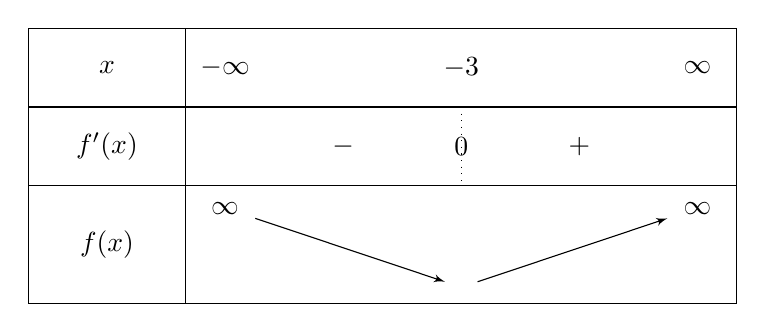
\begin{tikzpicture}
   \tkzTabInit{$x$ / 1 , $f'(x)$ / 1, $f(x)$ / 1.5}{$-\infty$, $-3$, $\infty$}
   \tkzTabLine{, -, z, +, }
   \tkzTabVar{ +/ $\infty$, -/ , +/$\infty$ }
\end{tikzpicture}
\end{center}
\item $f:x \mapsto \frac17x^2 + \frac23 x - \pi \quad ; \quad f'(x) = \frac27x + \frac23 \et f'(x) = 0 \iff x = -\frac73$. \newline
On remarque que $f'(0)= \frac23 >0$
\begin{center}
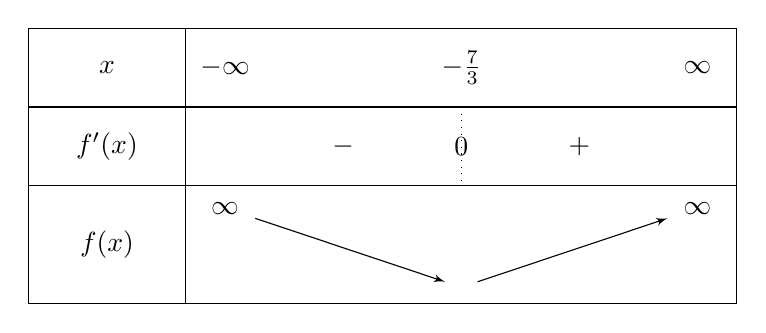
\begin{tikzpicture}
   \tkzTabInit{$x$ / 1 , $f'(x)$ / 1, $f(x)$ / 1.5}{$-\infty$, $-\frac73$, $\infty$}
   \tkzTabLine{, -, z, +, }
   \tkzTabVar{ +/ $\infty$, -/ , +/$\infty$ }
\end{tikzpicture}
\end{center}
\item Dans certains cas, les variations sont inversées, par exemple pour la fonction : \newline
$f : x \mapsto -2x^2 + 12x -2 \quad ; \quad f'(x) = -4x +12 \et f'(x) = 0 \iff x=3$. On remarque que $f'(1) = -4+12 = 8$ donc :
\begin{center}
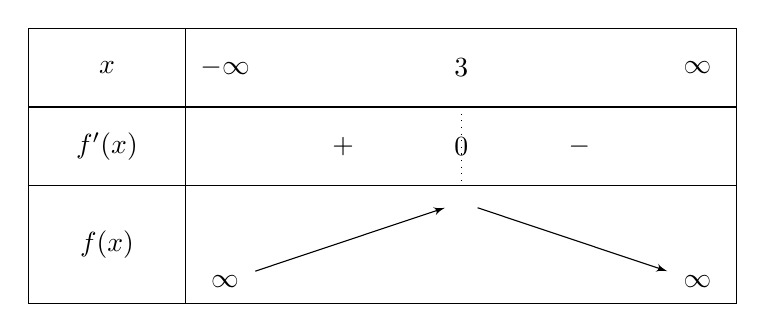
\begin{tikzpicture}
   \tkzTabInit{$x$ / 1 , $f'(x)$ / 1, $f(x)$ / 1.5}{$-\infty$, $3$, $\infty$}
   \tkzTabLine{, +, z, -, }
   \tkzTabVar{ -/ $\infty$, +/ , -/$\infty$ }
\end{tikzpicture}
\end{center}
On peut même calculer le maximum de $f$, qui est atteint en $3$ et qui vaut : 
\[ f(3) = -2 \cdot (3)^2 +12 \cdot 3 -2 = 16. \]
\end{enumerate}
}{exe:2}{

}
\newpage

\exe{}{
Pour étudier les variations de ce type de fonction, on procède excatement comme dans l'exercice 2, 
sauf que la recherche des valeurs $x$ telles que $f'(x)=0$ sera différente.
\begin{enumerate}
\item On étudie les variations de la fonction $f : x \mapsto 2x-12 + \frac{162}{x}$.
On a $f'(x) = 2 - \frac{162}{x^2}$. On cherche $x$ tel que $f'(x) = 0$. 
\begin{align*}
f'(x) = 0 & \iff 2 - \dfrac{162}{x^2} = 0 \\
& \iff \dfrac{2x^2}{x^2} -  \dfrac{162}{x^2} = 0 \\
& \iff \dfrac{2x^2-162}{x^2} = 0 \\
& \iff 2x^2-162 = 0 \\
& \iff 2x^2 = 162 \\
& \iff x^2 = 81 \\
& \iff x=-9 \text{~ou~} x=9 
\end{align*}
On a donc deux valeurs de $x$ pour lesquelles $f'(x)=0$.
On doit aussi se souvenir que $0$ est une valeur interdite (on la délimite avec deux barres dans le tableau).
Enfin, on remarque que $f'(1)=2-162<0$.
\begin{center}
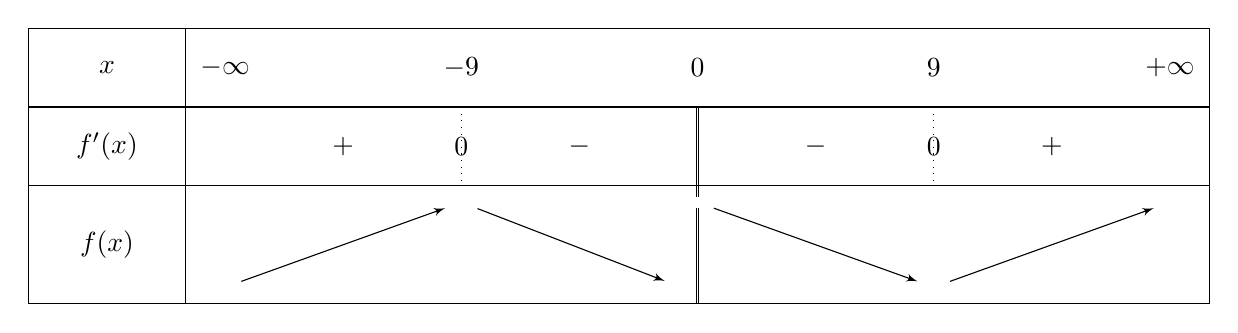
\begin{tikzpicture}
   \tkzTabInit{$x$ / 1 , $f'(x)$ / 1, $f(x)$ / 1.5}{$-\infty$, $-9$, $0$, $9$, $+\infty$}
   \tkzTabLine{, +, z, -, d, -, z, +, }
   \tkzTabVar{-/ , +/, -DC+/, -/, +/ }
\end{tikzpicture}
\end{center}
\item $f: x \mapsto 7x - 426 - \frac{2}{x}$, ici $f'(x) = 7 + \frac2{x^2}$ donc on remarque que $f'(x) \geq 2$ pour tout $x$.
On peut dresser directement le tableau :
\begin{center}
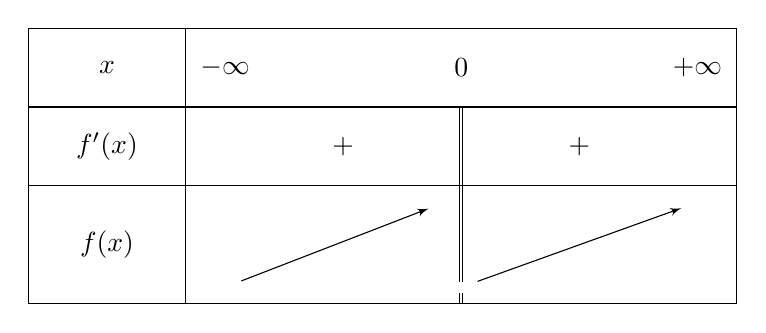
\begin{tikzpicture}
   \tkzTabInit{$x$ / 1 , $f'(x)$ / 1, $f(x)$ / 1.5}{$-\infty$, $0$, $+\infty$}
   \tkzTabLine{, +, d, +, }
   \tkzTabVar{-/ , +DC-/, +/ }
\end{tikzpicture}
\end{center}
\item $f:x \mapsto -10x + 20 - \frac{360}{x} \quad ; \quad f'(x) = -10 + \frac{360}{x^2}$ et 
\begin{align*}
f'(x) = 0 & \iff -10 + \dfrac{360}{x^2} = 0 \\
& \iff \dfrac{-10x^2}{x^2} +  \dfrac{360}{x^2} = 0 \\
& \iff \dfrac{-10x^2+360}{x^2} = 0 \\
& \iff -10x^2 + 360 = 0 \\
& \iff x^2 = 36 \\
& \iff x=-6 \text{~ou~} x=6 
\end{align*}
On remarque que $f'(1)=-10+360>0$.
\begin{center}
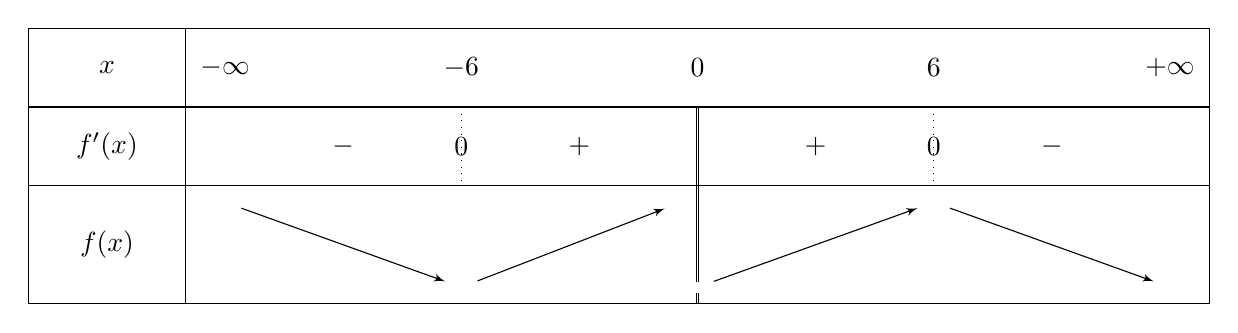
\begin{tikzpicture}
   \tkzTabInit{$x$ / 1 , $f'(x)$ / 1, $f(x)$ / 1.5}{$-\infty$, $-6$, $0$, $6$, $+\infty$}
   \tkzTabLine{, -, z, +, d, +, z, -, }
   \tkzTabVar{+/ , -/, +DC-/, +/, -/ }
\end{tikzpicture}
\end{center}
\item $f:x \mapsto -7x + 312 + \frac{12}{x} \quad ; \quad f'(x) = -7 - \frac{12}{x^2}$. \newline
On remarque que $f'(x) \leq -7$ pour tout $x$.
\begin{center}
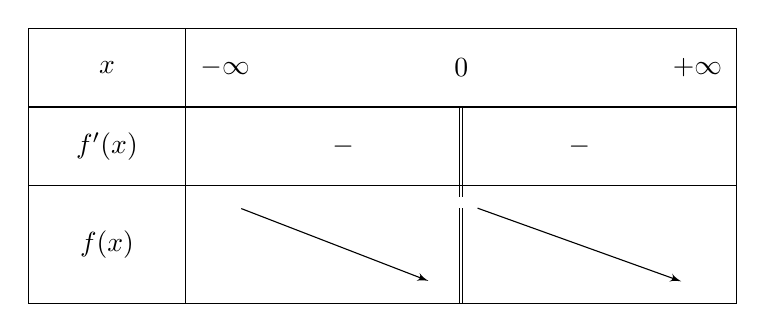
\begin{tikzpicture}
   \tkzTabInit{$x$ / 1 , $f'(x)$ / 1, $f(x)$ / 1.5}{$-\infty$, $0$, $+\infty$}
   \tkzTabLine{, -, d, -, }
   \tkzTabVar{+/ , -DC+/, -/ }
\end{tikzpicture}
\end{center}
\end{enumerate}
}{exe:3}{

}

\end{document}